\documentclass{standalone}
\usepackage{pgfplots}
\pgfplotsset{compat=1.17}
\usepackage{amsmath, amssymb, amsbsy, amstext, amsthm, simplewick}
\usepackage{physics}
\usepackage{bm}
\usepackage{siunitx}
\usepackage[acronym]{glossaries}

%% Abbreviations
\newcommand{\eg}{{e.g.}}
\newcommand{\ie}{{i.e.}}

%% Statistics
\newacronym{lbi}{LBI}{likelihood-based inference}
\newacronym{sbi}{SBI}{simulation-based inference}
\newacronym{abc}{ABC}{approximate Bayesian computation}
\newacronym{kl}{KL}{Kullback-Leibler}
\newacronym{vi}{VI}{variational inference}
\newacronym{npe}{NPE}{neural posterior estimation}
\newacronym{nle}{NLE}{neural likelihood estimation}
\newacronym{nre}{NRE}{neural ratio estimation}
\newacronym{mnre}{MNRE}{marginal neural ratio estimation}
\newacronym{tmnre}{TMNRE}{truncated marginal neural ratio estimation}
\newacronym{mcmc}{MCMC}{Markov-chain Monte Carlo}
\newacronym{hmc}{HMC}{Hamiltonian Monte Carlo}
\newacronym{snr}{SNR}{signal-to-noise}
\newacronym{ps}{PS}{power spectrum}
\newacronym{mlr}{MLR}{maximum likelihood ratio}
\newacronym{nn}{NN}{neural network}
\newacronym{cnn}{CNN}{convolutional neural network}
\newacronym{gan}{GAN}{generative adversarial network}
\newacronym{vit}{ViT}{Vision Transformer}
\newacronym{mlp}{MLP}{multilayer perceptron}
\newacronym{bce}{BCE}{binary cross-entropy}

\newcommand{\swyft}{\textit{swyft} }

%% Physics
\newacronym{los}{LOS}{line-of-sight}
\newacronym{nfw}{NFW}{Navarro-Frenk-White}
\newacronym{psf}{PSF}{point-spread function}
\newacronym{shmf}{SHMF}{subhalo mass function}
\newacronym{sie}{SIE}{singular isothermal ellipsoid}
\newacronym{sple}{SPLE}{singular power law ellipsoid}
\newacronym{gr}{GR}{general relativity}
\newacronym{dm}{DM}{dark matter}
\newacronym{cdm}{CDM}{cold dark matter}
\newacronym{wdm}{WDM}{warm dark matter}
\newacronym{hmf}{HMF}{halo mass function}
\newacronym{hst}{HST}{Hubble Space Telescope}


%% Units
\DeclareSIUnit \Mpc {Mpc}
\DeclareSIUnit \arcsec {arcsec}
\DeclareSIUnit \solmass {M_{\odot}}
\newcommand{\keV}{\kiloElectronvolt}

%% Distributions
\newcommand{\Uniform}{\mathcal{U}}
\newcommand{\Normal}{\mathcal{N}}

%% Parameters
\newcommand{\data}{\ensuremath{\bm{x}}}
\newcommand{\param}{\ensuremath{\bm{\Theta}}}
\newcommand{\interest}{\ensuremath{\bm{\theta}}}
\newcommand{\nuisance}{\ensuremath{\bm{\eta}}}

\newcommand{\plens}{\ensuremath{\nuisance_\mathrm{lens}}}
\newcommand{\psrc}{\ensuremath{\nuisance_\mathrm{src}}}
\newcommand{\msub}{\ensuremath{\bm{m}_{200, \mathrm{sub}}}}
\newcommand{\mlos}{\ensuremath{\bm{m}_{200, \mathrm{los}}}}
\newcommand{\psubb}{\ensuremath{{{\nuisance}}_\mathrm{sub}}}
\newcommand{\psub}{\ensuremath{\vec{{\nuisance}}_\mathrm{sub}}}
\newcommand{\plos}{\ensuremath{\vec{{\nuisance}}_\mathrm{los}}}
\newcommand{\pp}{\ensuremath{\boldsymbol{\vec{{\nuisance}}_\mathrm{p}}}}
\newcommand{\zlos}{\ensuremath{\bm{z}_\mathrm{los}}}
\newcommand{\mhm}{\ensuremath{\mathrm{M_{hm}}}}

\newcommand{\hypgeom}{\ensuremath{{}_2\mathrm{F}_1}}

%%%%%%%%%%%%%%%%% Define Lots of Random Colors %%%%%%%%%%%%%%%%%%%%

\definecolor{silver}{rgb}{0.75, 0.75, 0.75}
\definecolor{myblue}{rgb}{0,0.298,0.49}
\definecolor{mauve}{rgb}{0.25, 0.41, 0.88}
\definecolor{red}{rgb}{0.92,0.,0.}
\definecolor{orange}{rgb}{1.0,0.549,0.}
\definecolor{bluegray}{rgb}{0.368417, 0.506779, 0.709798}
\definecolor{lightorange}{rgb}{0.880722, 0.611041, 0.142051}
\definecolor{grassgreen}{rgb}{0.560181, 0.691569, 0.194885}
\definecolor{violet}{rgb}{0.528488, 0.470624, 0.701351}
\definecolor{lightblue}{rgb}{0.363898, 0.618501, 0.782349}
\definecolor{yellow}{rgb}{1, 0.75, 0}
\definecolor{purple}{rgb}{0.647624, 0.37816, 0.614037}
\definecolor{blue}{HTML}{0068AC}
\definecolor{varpurple}{rgb}{0.431,0.188,0.534}
\definecolor{darkgreen}{rgb}{0.075,0.302,0.047}
\definecolor{darkergreen}{rgb}{0,0.294,0.188}
\definecolor{dullred}{rgb}{0.706,0.208,0.192}
\definecolor{darkred}{rgb}{0.545,0,0}
\definecolor{antiquefuchsia}{rgb}{0.57, 0.36, 0.51}
\definecolor{teal}{rgb}{0,0.502,0.502}
\definecolor{dullblue}{rgb}{0,0.298,0.49}
\definecolor{green}{RGB}{44, 160, 44}


\begin{document}

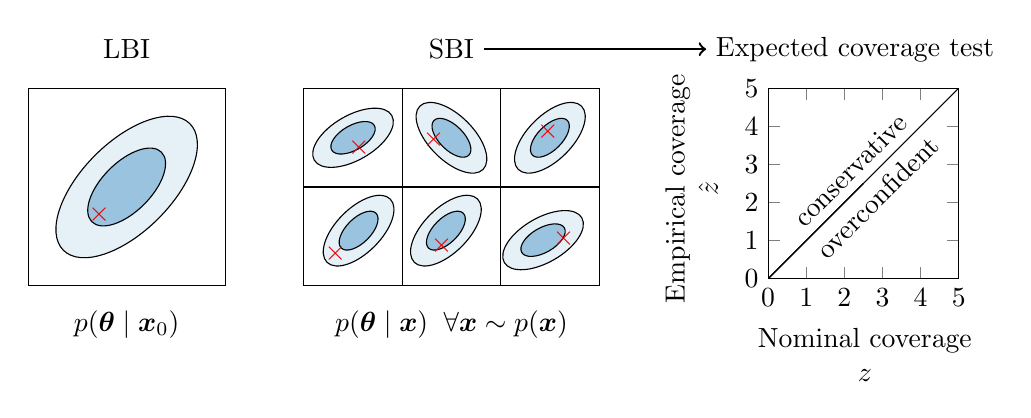
\begin{tikzpicture}

    \pgfmathsetmacro{\squareSize}{2.5}
    \pgfmathsetmacro{\offset}{1} 

    % Draw the first region with one square
    \draw (0, 0) rectangle ++(\squareSize, \squareSize);
    \draw[fill=blue!10,rotate around={45:(\squareSize/2, \squareSize/2)}] (\squareSize/2, \squareSize/2) ellipse (\squareSize/2/1.1 and \squareSize/2/2.2); 
    \draw[fill=blue!40,rotate around={45:(\squareSize/2, \squareSize/2))}] (\squareSize/2, \squareSize/2) ellipse (\squareSize/2/2 and \squareSize/2/4);
    \node[] at (0.9, 0.9){\color{red} $\times$ };
    \node (lbi) at (\squareSize/2, \squareSize+0.5) {LBI};
    \node at (\squareSize/2, -0.5) {$p(\interest\mid\data_0)$};
    
    % Draw the central region with two squares
    \draw (\squareSize+\offset, 0) rectangle ++(\squareSize/2, \squareSize/2);
    \draw[fill=blue!10,rotate around={45:(\squareSize+\offset+\squareSize/4, \squareSize/4)}] (\squareSize+\offset+\squareSize/4+0.1,\squareSize/4) ellipse (\squareSize/4/1.1 and \squareSize/4/2.2); 
    \draw[fill=blue!40,rotate around={45:(\squareSize+\offset+\squareSize/4, \squareSize/4)}] (\squareSize+\offset+\squareSize/4+0.1,\squareSize/4) ellipse (\squareSize/4/2 and \squareSize/4/4);
    \node[] at (\squareSize+\offset+0.4, 0.4){\color{red} $\times$ };     
    \draw (\squareSize+\offset, \squareSize/2) rectangle  ++(\squareSize/2, \squareSize/2);
    \draw[fill=blue!10,rotate around={30:(\squareSize+\offset+\squareSize/4, \squareSize/2+\squareSize/4)}] (\squareSize+\offset+\squareSize/4,\squareSize/2+\squareSize/4) ellipse (\squareSize/4/1.1 and \squareSize/4/2.2); 
    \draw[fill=blue!40,rotate around={30:(\squareSize+\offset+\squareSize/4, \squareSize/2+\squareSize/4)}] (\squareSize+\offset+\squareSize/4,\squareSize/2+\squareSize/4) ellipse (\squareSize/4/2 and \squareSize/4/4);
    \node[] at (\squareSize+\offset+0.7, \squareSize/2+0.5){\color{red} $\times$ };
    \draw (\squareSize+\offset+\squareSize/2, 0) rectangle  ++(\squareSize/2, \squareSize/2);
    \draw[fill=blue!10,rotate around={45:(\squareSize+\offset+\squareSize/4+\squareSize/2, \squareSize/4)}] (\squareSize+\squareSize/2+\offset+\squareSize/4,\squareSize/4+0.1) ellipse (\squareSize/4/1.1 and \squareSize/4/2.2); 
    \draw[fill=blue!40,rotate around={45:(\squareSize+\offset+\squareSize/4+\squareSize/2, \squareSize/4)}] (\squareSize+\squareSize/2+\offset+\squareSize/4,\squareSize/4+0.1) ellipse (\squareSize/4/2 and \squareSize/4/4);
    \node[] at (\squareSize+\offset+\squareSize/2+0.5, 0.5){\color{red} $\times$ };
    \draw (\squareSize+\offset+\squareSize/2, \squareSize/2) rectangle  ++(\squareSize/2, \squareSize/2);
    \draw[fill=blue!10,rotate around={-45:(\squareSize+\offset+\squareSize/4+\squareSize/2, \squareSize/4+\squareSize/2)}] (\squareSize+\squareSize/2+\offset+\squareSize/4,\squareSize/4+\squareSize/2) ellipse (\squareSize/4/1.1 and \squareSize/4/2.2); 
    \draw[fill=blue!40,rotate around={-45:(\squareSize+\offset+\squareSize/4+\squareSize/2, \squareSize/4+\squareSize/2)}] (\squareSize+\squareSize/2+\offset+\squareSize/4,\squareSize/4+\squareSize/2) ellipse (\squareSize/4/2 and \squareSize/4/4);
    \node[] at (\squareSize+\offset+\squareSize/2+0.4, \squareSize/2+0.6){\color{red} $\times$ };
    \draw (2*\squareSize+\offset, 0) rectangle  ++(\squareSize/2, \squareSize/2);
    \draw[fill=blue!10,rotate around={30:(2*\squareSize+\offset+\squareSize/4, \squareSize/4)}] (2*\squareSize+\offset+\squareSize/4-0.1,\squareSize/4) ellipse (\squareSize/4/1.1 and \squareSize/4/2.2); 
    \draw[fill=blue!40,rotate around={30:(2*\squareSize+\offset+\squareSize/4, \squareSize/4)}] (2*\squareSize+\offset+\squareSize/4-0.1,\squareSize/4) ellipse (\squareSize/4/2 and \squareSize/4/4);
    \node[] at (2*\squareSize+\offset+0.8, 0.6){\color{red} $\times$ };
    \draw (2*\squareSize+\offset, \squareSize/2) rectangle  ++(\squareSize/2, \squareSize/2);
    \draw[fill=blue!10,rotate around={45:(2*\squareSize+\offset+\squareSize/4, \squareSize/4+ \squareSize/2)}] (2*\squareSize+\offset+\squareSize/4,\squareSize/4+ \squareSize/2) ellipse (\squareSize/4/1.1 and \squareSize/4/2.2); 
    \draw[fill=blue!40,rotate around={45:(2*\squareSize+\offset+\squareSize/4, \squareSize/4+ \squareSize/2)}] (2*\squareSize+\offset+\squareSize/4,\squareSize/4+ \squareSize/2) ellipse (\squareSize/4/2 and \squareSize/4/4);
    \node[] at (2*\squareSize+\offset+0.6, \squareSize/2+0.7){\color{red} $\times$ };
    \node (sbi) at (\squareSize+\offset+\squareSize*0.75, \squareSize+0.5) {SBI};
    \node (all) at (\squareSize+\offset+\squareSize*0.75, -0.5) {$p(\interest\mid\data)\;\; \forall \data\sim p(\data)$};

    % Draw the third region with one square
    \node (test) at (3*\squareSize+2*\offset+1, \squareSize+0.5) {Expected coverage test};
    \draw[->, line width=0.3mm, draw=black] (sbi.east) to (test.west);
    \begin{axis}[
    		width=0.33\linewidth, height=0.33\linewidth, at={(0.775*\linewidth, 0.007*\linewidth)},
			xmax=5, xmin=0,
			ymax=5, ymin=0,
			xtick={0,1,2,3,4,5},
		    ytick={0,1,2,3,4,5},
    	]
    	\addplot [black,samples at={0,5}] {x};
    	\draw (axis cs:0,0)--(axis cs:2.5,2.5) node [anchor=south, rotate=45]{conservative};
    	\draw (axis cs:0,0)--(axis cs:2.5,2.5) node [anchor=north, rotate=45]{overconfident};
    \end{axis}
    \node [label={[align=center]below:Nominal coverage\\ ${z}$}] (n) at (4.25*\squareSize,-0.3) {};
    \node [rotate=90,label={[align=center, rotate=90]below:Empirical coverage\\ $\hat{z}$} ] (e) at (3*\squareSize+0.8, -0.35){};
   
    
\end{tikzpicture}


\end{document}
